%\title{LaTeX Portrait Poster Template}
%%%%%%%%%%%%%%%%%%%%%%%%%%%%%%%%%%%%%%%%%
% a0poster Portrait Poster
% LaTeX Template
% Version 1.0 (22/06/13)
%
% The a0poster class was created by:
% Gerlinde Kettl and Matthias Weiser (tex@kettl.de)
% 
% This template has been downloaded from:
% http://www.LaTeXTemplates.com
%
% License:
% CC BY-NC-SA 3.0 (http://creativecommons.org/licenses/by-nc-sa/3.0/)
%
%%%%%%%%%%%%%%%%%%%%%%%%%%%%%%%%%%%%%%%%%

%----------------------------------------------------------------------------------------
%	PACKAGES AND OTHER DOCUMENT CONFIGURATIONS
%----------------------------------------------------------------------------------------

\documentclass[a0,portrait]{a0poster}

\usepackage{multicol} % This is so we can have multiple columns of text side-by-side
\columnsep=100pt % This is the amount of white space between the columns in the poster
\columnseprule=3pt % This is the thickness of the black line between the columns in the poster

\usepackage[svgnames]{xcolor} % Specify colors by their 'svgnames', for a full list of all colors available see here: http://www.latextemplates.com/svgnames-colors

\usepackage{times} % Use the times font
%\usepackage{palatino} % Uncomment to use the Palatino font

\usepackage{graphicx} % Required for including images
\graphicspath{{figures/}} % Location of the graphics files
\usepackage{booktabs} % Top and bottom rules for table
\usepackage[font=small,labelfont=bf]{caption} % Required for specifying captions to tables and figures
\usepackage{amsfonts, amsmath, amsthm, amssymb} % For math fonts, symbols and environments
\usepackage{wrapfig} % Allows wrapping text around tables and figures
\usepackage{tikz}
\usepackage{titlesec}
\usepackage{lipsum}% http://ctan.org/pkg/lipsum
%\usepackage{showframe}% http://ctan.org/pkg/showframe
\usepackage{eso-pic}% http://ctan.org/pkg/eso-pic
\usepackage{graphicx}% http://ctan.org/pkg/graphicx

\begin{document}

\newcommand*{\justifyheading}{\raggedleft}
%----------------------------------------------------------------------------------------
%	POSTER HEADER 
%----------------------------------------------------------------------------------------

% The header is divided into two boxes:
% The first is 75% wide and houses the title, subtitle, names, university/organization and contact information
% The second is 25% wide and houses a logo for your university/organization or a photo of you
% The widths of these boxes can be easily edited to accommodate your content as you see fit
\begin{minipage}[b]{0.15\linewidth}

\includegraphics[width=10cm]{uni_logo.png}\\
\end{minipage}
%\addtobeamertemplate{headline}{} 

\begin{minipage}[!b]{0.85\linewidth}
\VeryHuge\justifyheading \color{NavyBlue} \textbf{Weather Classification with Deep Learning} \color{Black}\\ % Title
%\Huge\textit{Country Update}\\[2.4cm] % Subtitle

%\vspace{1cm} % A bit of extra whitespace between the header and poster content

\huge \textbf{Junjie Zhang}\\[0.6cm] % Author(s)
\huge Advisor: Profesor Chunhua Shen \\[0.5cm] % advisor
\huge The University of Adelaide, School of Computer Science \\[0.5cm] % University/organization
\end{minipage}
%

%----------------------------------------------------------------------------------------
\begin{multicols}{2} % This is how many columns your poster will be broken into, a portrait poster is generally split into 2 columns


%----------------------------------------------------------------------------------------
%	ABSTRACT
%----------------------------------------------------------------------------------------

%\color{Navy} % Navy color for the abstract

\begin{abstract}
Scene classification is an important field in computer vision. For similar weather condition, there are some obstacles for extracting features from outdoor images. We present a novel approach to classify cloudy and sunny weather. Inspired by recent study of deep convolutional neural network(CNN) and spatial pyramid polling, we generate a model based on ImageNet dataset. Starting with parameters trained from more than 1 million images, we fine-tune the parameters. Experiment demonstrates that our classifier can achieve the state of the art accuracy.
\end{abstract}

\section*{Introduction}
As usually defined, image understand by a machine can be seen as an attempt to find a relation between input images and previously established models of the observed world~\cite{sonka1998image}.One of scenario is understanding weather conditions. People usually judge weather by views, and bureau of meteorology uses special complex instruments, which include satellite. These approaches are labour consuming and expensive. In this paper, we state a computational approach to classify two similar weather conditions-sunny and cloudy.

Some obstacles are in front of weather classification. First of all, sunny and cloudy are similar weather conditions. There are no decisive features, say brightness and lightness, to classify them. Second, it is not easy to extract middle level features and follow a set of decision rules to put a image into a category. For example, shade can be found in sunny and cloudy weather. Last but not least, outdoor images are various.

%----------------------------------------------------------------------------------------
%	DATASETS AND METHODS
%----------------------------------------------------------------------------------------

\section*{Datasets and Methods}

The datasets for training CNN is from ImageNet, there are more than 1 million images in 1000 categories. 
The datasets for fine-tuning are from \cite{lutwo}. There are 10,000 images. The half are cloudy and other half are sunny. We take out 1000 images randomly for testing and 9000 images for training.
We will achieve the objective with following method.
\begin{enumerate}
\item Implement spatial pyramid match layer.
\item Train CNN model with ImageNet dataset.
\item Fine tune model with weather images.
\end{enumerate}

\subsection*{Mathematical and Diagrams}

For a multilayer neural networks, the mathematical representation can be represented as

\begin{equation}\label{eq:ffEq}
y_{m} = \hat{f}\Big(\sum_{j=0}^{m}w_{j4}^{(2)}f\big(\sum_{i=0}^{n}w_{4i}^{(1)}x_{i}\big)\Big)
\end{equation}
In the \ref{eq:ffEq}, outer activation function could be different with the inner one.

We use the architecture which achieved excellent performance in 2012 ImageNet classification competition. 

\begin{center}\vspace{1cm}
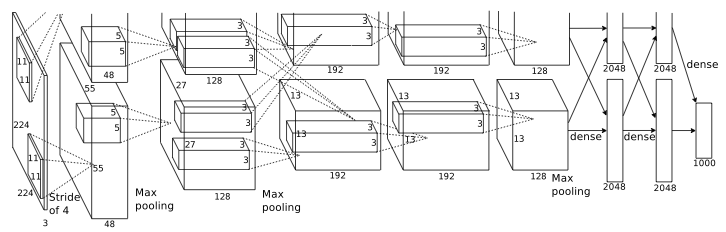
\includegraphics[width=0.8\linewidth]{figures/AlexNet.png}
\captionof{figure}{\color{Green} Architecture of CNN}
\end{center}\vspace{1cm}

Backpropagation is a method of training CNN used with an optimization method. It can be represent as

\begin{equation}\label{eq:h2oBP}
\Delta w(jk) = -\eta \frac{\partial E}{\partial w_{jk}} = -\eta \delta_{k}y_{j}
\end{equation}
where $$\delta_{k} = \frac{\partial E}{\partial a_{k}} = (y_{k} - t_{k})y_{k}(1 - y_{k})$$

Spatial pyramid match\cite{lazebnik2006beyond} is used to classify high-level semantic attributes, based on low-level features. The method subdivides a image in several different levels of resolution and counts features falling in each spatial bin. It extends bags of features and derives spatial information from images.

\begin{center}\vspace{1cm}
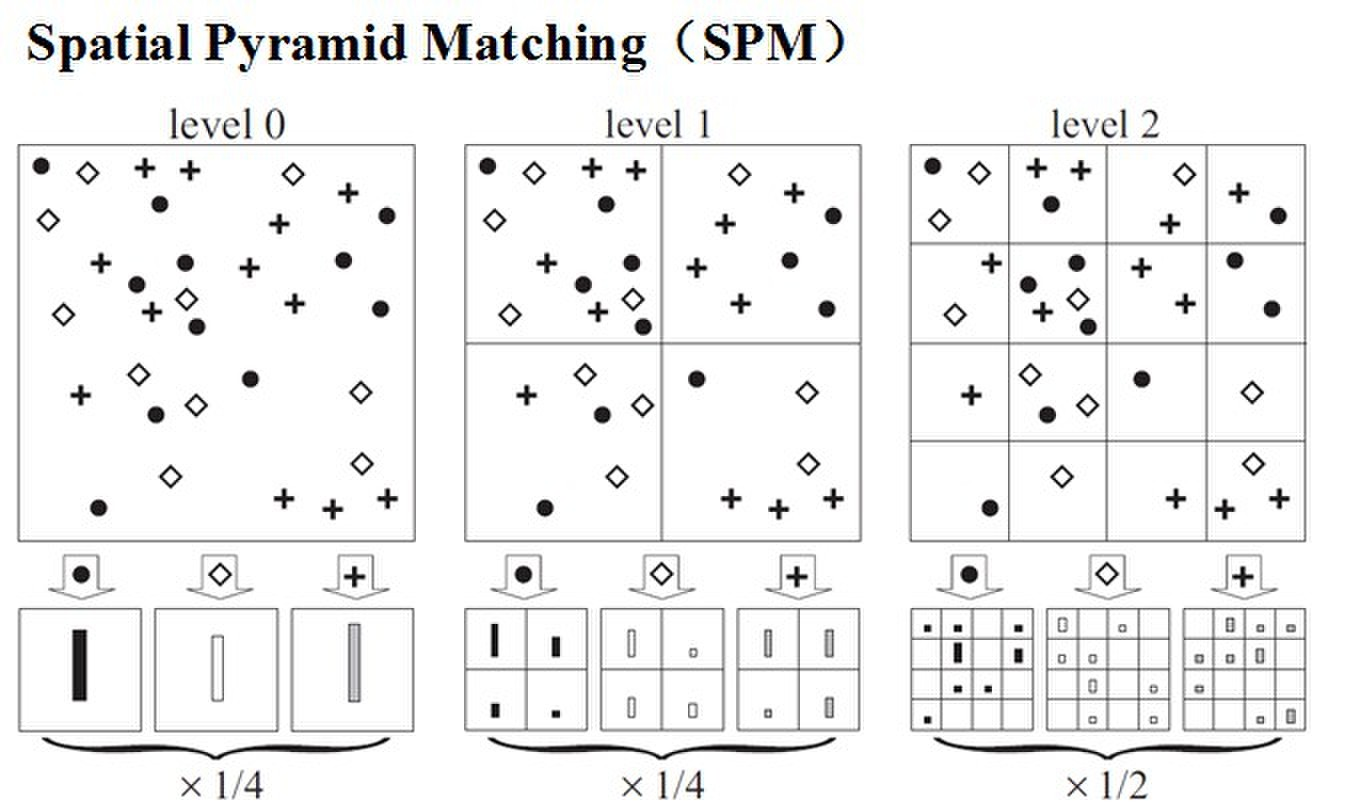
\includegraphics[width=0.8\linewidth]{figures/spm.jpg}
\captionof{figure}{\color{Green} Diagram of Spatial Pyramid Match.}
\end{center}\vspace{1cm}
 
SPM can be represented as

\begin{align*}
\kappa^{L}(X,Y) &= \mathcal{I}^{L} + \sum_{l=0}^{L-1}\frac{1}{{2}^{L-l}}(\mathcal{I}^{l}-\mathcal{I}^{l+1})\\
 & = \frac{1}{2^{L}}\mathcal{I}^{0} + \sum_{l=1}^{L}\frac{1}{2^{L-l+1}}\mathcal{I}^{l}
\end{align*}

%----------------------------------------------------------------------------------------
%	RESULTS 
%----------------------------------------------------------------------------------------

\section*{Results}

We can see from Table \ref{result} that the model has an excellent performance on two class weather classification. The methods CNN+SVM and SPP+SVM mean that we extract features from pretrained models and train linear SVM classifiers. The next two methods fine tune pretrained models with weather images. 

%
\begin{center}
\begin{tabular}{c c c c}
\toprule
\textbf{CNN+SVM} & \textbf{SPP+SVM} & \textbf{Finetune on CNN}& \textbf{Finetune on SPP}\\
\midrule
$84.8\%$ & $82.1\%$ & $93.1\%$ & $93.98\%$ \\

\bottomrule
\label{result}
\end{tabular}
\captionof{table}{\color{Green} Classification Accuracy}
\end{center}

%----------------------------------------------------------------------------------------
%	Analysis
%----------------------------------------------------------------------------------------

\section*{Analysis}

Some intuition on how CNN works.
\begin{center}\vspace{1cm}
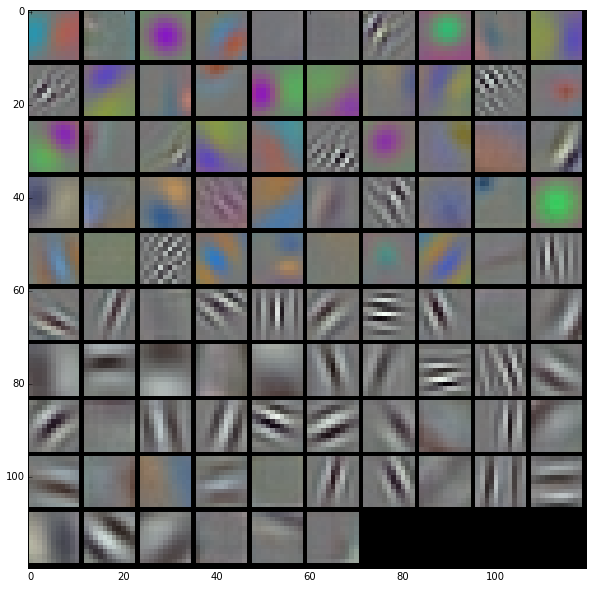
\includegraphics[width=0.3\linewidth]{conv1_params.png}
\captionof{figure}{\color{Green} 36 filters in the first convolutional layer}
\end{center}\vspace{1cm}

Then we can use the filters to transform original images and compare the outputs.

\begin{center}\vspace{1cm}
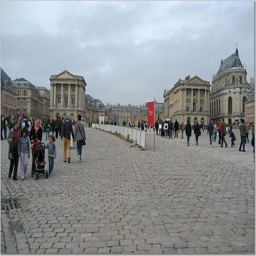
\includegraphics[width=0.3\linewidth]{cloudy1}
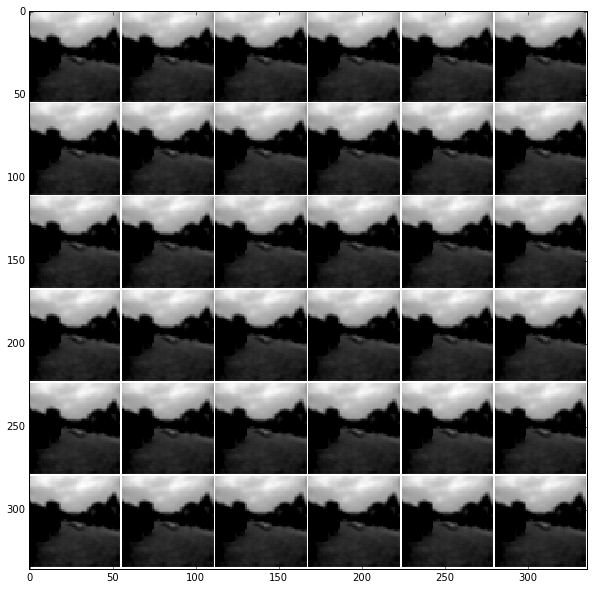
\includegraphics[width=0.3\linewidth]{cloudy1_conv1_fm}
\captionof{figure}{\color{Green} A cloudy image and outputs of the first layer}
\end{center}\vspace{1cm}

\begin{center}\vspace{1cm}
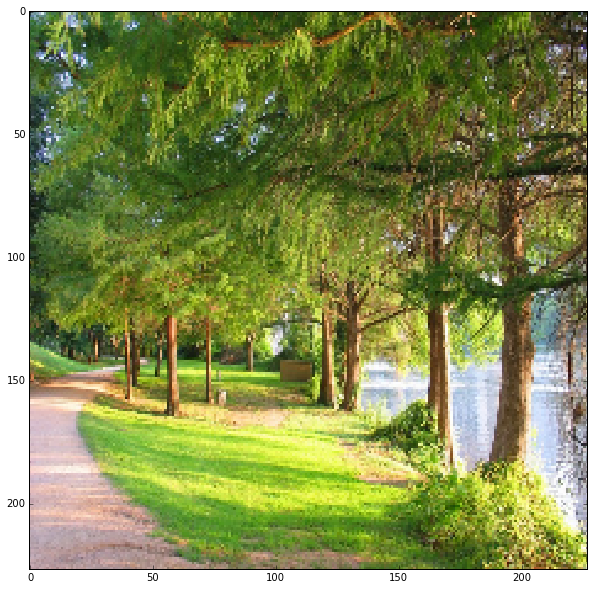
\includegraphics[width=0.3\linewidth]{sunny2}
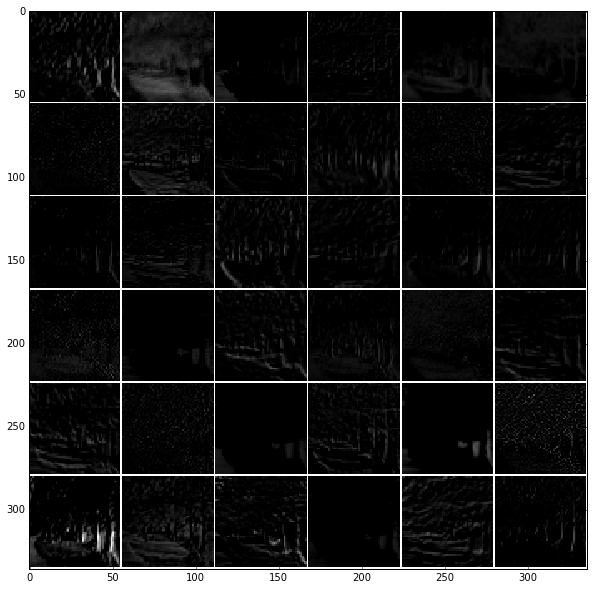
\includegraphics[width=0.3\linewidth]{sunny2_conv1_fm}
\captionof{figure}{\color{Green} A sunny image and outputs of the first layer}
\end{center}\vspace{1cm}

%----------------------------------------------------------------------------------------
%	CONCLUSIONS
%----------------------------------------------------------------------------------------

%\color{SaddleBrown} % SaddleBrown color for the conclusions to make them stand out

\section*{Conclusions}

\begin{itemize}
\item CNN has power capability of recognizing images.
\item Fine tune can save computation in terms of time and power, reducing from one week to one day.
\item Fine tune can reduce overfitting risk. 
\end{itemize}

%\color{DarkSlateGray} % Set the color back to DarkSlateGray for the rest of the content

%----------------------------------------------------------------------------------------
%	FORTHCOMING RESEARCH
%----------------------------------------------------------------------------------------

\section*{Forthcoming Research}

Although CNN achieve success in image classification, we still have little knowledge of why and how it works. In future research, we will focus on analysing working mechanism of deep layers and the interaction between data and model.

%----------------------------------------------------------------------------------------
%	REFERENCES
%----------------------------------------------------------------------------------------

%\nocite{*} % Print all references regardless of whether they were cited in the poster or not
\bibliographystyle{plain} % Plain referencing style
\bibliography{sample} % Use the example bibliography file sample.bib


\end{multicols}
\end{document}